%!TEX root = ../3dbook.tex

\setchapterpreamble[u]{\margintoc}

\graphicspath{{curves/}}
% \renewcommand*{\thelesson}{6.1}

\chapter{B\'ezier curves and surfaces}
\label{chap:curves}

The vast majority of geographic information uses only linear geometries (\ie\ line segments, polygons and polyhedra).
When curved geometries are present, they are usually simple parametric shapes, such as spheres, cylinders and cones in CSG or circular arcs in certain 2D datasets (Figure~\ref{fig:circulararc}).
Moreover, most data models are designed with linear geometries in mind.

\begin{marginfigure}
\centering
\includegraphics[width=0.8\linewidth]{figs/circulararc}
\caption{A composite curve made from two line segments and a circular arc.}%
\label{fig:circulararc}
\end{marginfigure}

However, modelling curves and curved surfaces is still highly desirable in certain circumstances, as they make it possible to model many shapes a lot more compactly and without losing precision through discretisation.
Most CAD and 3D modelling software thus support curves and curved surfaces, and BIM models routinely use them internally as well.

There are several methods that can be used to represent general curves in 2D/3D and curved surfaces in 3D.
This chapter covers one of them that is relatively simple and works well in practice: B\'ezier curves and surfaces.

\section{Background}

\subsection{Types of points}

In general, curve and surface modelling is done by specifying the locations of points, of which there are two kinds (Figure~\ref{subfig:pointtypesa}):

\begin{figure}
\centering
\begin{subfigure}{0.5\linewidth}
\includegraphics[width=\linewidth]{figs/pointtypesa}
\caption{}%
\label{subfig:pointtypesa}
\end{subfigure}%
\begin{subfigure}{0.4\linewidth}
\includegraphics[width=\linewidth]{figs/pointtypesb}
\caption{}%
\label{subfig:pointtypesb}
\end{subfigure}\\
\caption{(a) The data points (white) and control points (black) used to draw a B\'ezier curve.
(b) In Affinity Designer (shown here) and most other graphics editors, data points (large circles) are surrounded by handles with the control points at their ends (small blue circles)}%
\label{fig:pointtypes}
\end{figure}

\begin{description}
\item[data points] are\marginnote{data point}\index{data point} points that the curve/surface needs to pass through; and
\item[control points] are\marginnote{control point}\index{control point} points that have some influence over the shape of the curve/surface, but through which the curve/surface does not necessarily pass. Intuitively, they `pull' the curve in their direction.
\end{description}

Note that in some contexts, they might all be referred to as control points (\eg\ graphics software), whereas in others (\eg\ interpolation) the distinction is almost always made.
If you have some experience with vector-based graphic editors (\eg\ Adobe Illustrator, Inkscape or Sketch), you have likely drawn curves using data points and control points (Figure~\ref{subfig:pointtypesb}).

\subsection{Types of curves and surfaces}

There are three kinds of mathematical representations that are typically used to represent curves and surfaces.
From most restrictive to least restrictive, these are:

\begin{description}
\item[Explicit curves/surfaces] are\marginnote{explicit curve}\index{explicit curve}\marginnote{explicit surface}\index{explicit surface} modelled using a function that defines the value of one coordinate, generally \(y\) in 2D and \(z\) in 3D, based on the other coordinate(s).
For instance, \(f(x)=y=x^2\) can be used to define a parabola in 2D, and \(f(x,y)=z=x^2+y^2\) to define a paraboloid in 3D.
This makes it impossible to represent vertical lines in 2D and planes in 3D (without swapping the dependent and independent variables in the equation), and makes it difficult to have multiple values per dependent variable, with minor exceptions such as the use of plus or minus (\(\pm\)), \eg\ \(f(x)=y = \pm\sqrt{1-x^2}\) for a circle or \(f(x,y)=z = \pm\sqrt{1-x^2-y^2}\) for a sphere.

\item[Implicit curves/surfaces] are\marginnote{implicit curve}\index{implicit curve}\marginnote{implicit surface}\index{implicit surface} modelled using a single function with all coordinates as parameters.
For instance, \(f(x,y) = x^2+y^2=1\) defines a unit circle in 2D and \(f(x,y,z)=x^2+y^2+z^2=1\) defines a unit sphere in 3D.
This works fine with vertical lines/planes and can represent multiple values per dependent variable, but completely functions have to be built to represent different curves.

\item[Parametric curves/surfaces] are\marginnote{parametric curve}\index{parametric curve}\marginnote{parametric surface}\index{parametric surface} modelled using different functions per coordinate which have independent non-coordinate variables as parameters.
For instance, \(f(t) = (\cos t, \sin t)\) with \(0 \leq t \leq 2\pi \) defines a unit circle in 2D, whereas \(f(t) = (\cos \theta \sin \phi , \sin \theta \sin \phi, \cos \phi)\) with \(0 \leq \theta \leq 2\pi \) and \(0 \leq \rho \leq \pi \) defines a unit sphere in 3D.
This is the most flexible approach because it allows us to define curves and surfaces in a general form that works independently of the coordinates used. 
\end{description}

Because of their flexibility, B\'ezier curves/surfaces and most other curve modelling methods (\eg\ splines) are based on parametric curves/surfaces.
For the rest of this chapter, we will therefore be working with parametric curves/surfaces only.

\subsection{Tangent vectors and other derivatives}

If we compute the first derivative of a parametric curve with respect to its parameter(s) at a given point, we get vector(s)\marginnote{tangent vector}\index{tangent vector} with a direction that is tangent to the curve and a magnitude that tells us the rate of change of the parameter(s) at that point.
For instance, in the curve \(C(x,y) = (\cos t, \sin t)\) with \(0 \leq t \leq 2\pi \) (Figure~\ref{fig:derivatives}), which describes the unit circle, at \(t=0\) we get the point \((1, 0)\), \ie\ the rightmost point on the circle using the typical axis directions.
The tangent vector is then \(dC(x,y)/dt = (-\sin t, \cos t)\), which at \(t=0\) is \((0, 1)\), \ie\ a unit vector pointing upwards (which makes sense considering that it draws the circle in a counter-clockwise direction).

\begin{marginfigure}
\centering
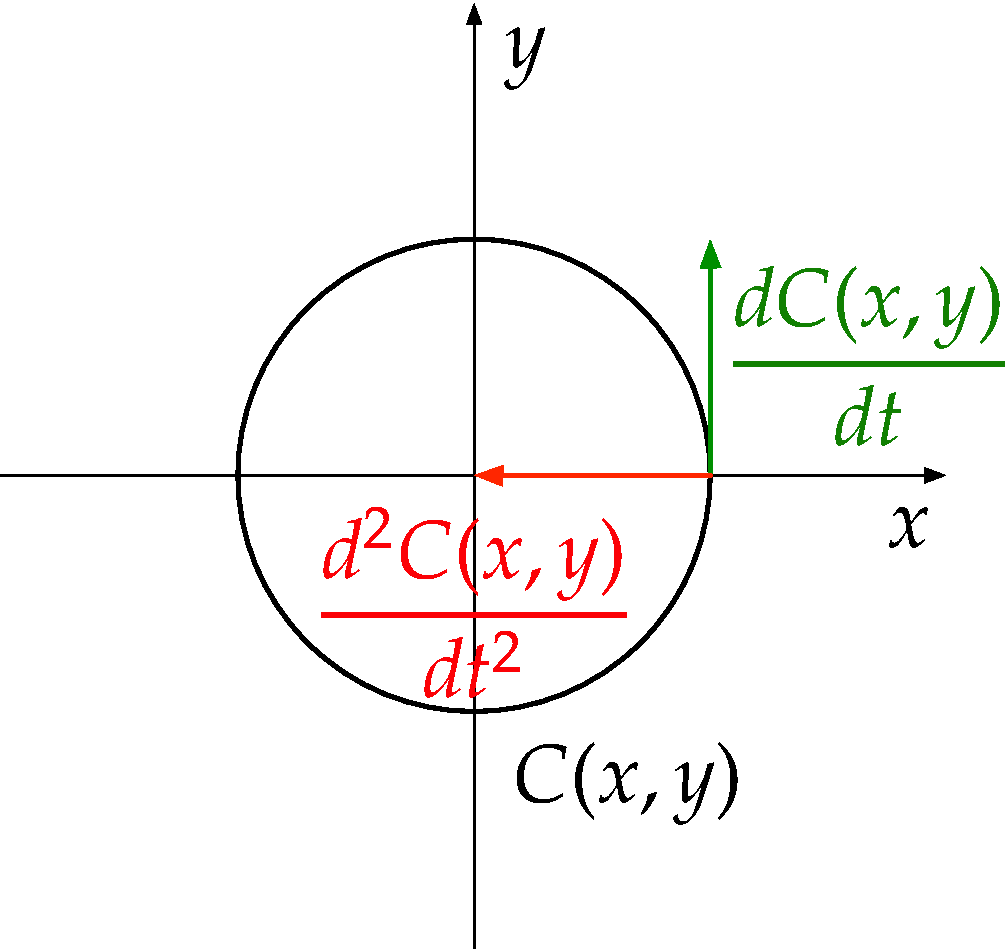
\includegraphics[width=\linewidth]{figs/derivatives}
\caption{The parametric curve \(C(x,y) = (\cos t, \sin t)\) for the unit circle (black), its first derivative at \(t=0\) (green), and the second derivative (red).}%
\label{fig:derivatives}
\end{marginfigure}

A common analogy to understand this concept is to consider a moving particle moving in time (hence you will often see \(t\) used in parametric functions).
The parametric function tells us the position of the particle at any given time, and the tangent vector tells us the direction and speed of the particle at that time.

The second derivative of a parametric curve is a little harder to visualise, but it is also a vector that tells us the rate of change of the curvature at a point.
In the particle analogy, it is the acceleration of the particle (and its acceleration direction).
In the circle from the previous example, the second derivative is \(d^2C(x,y)/dt^2 = (-\cos t, -\sin t)\), which at \(t=0\) is \((-1, 0)\), \ie\ a unit vector towards the centre of the circle.

\subsection{Uniform vs.\ non-uniform}

In order to fit a parametric curve through a series of points, we need to decide the curve equations and the values of the parameters that should be used.
We will discuss the curve equations for B\'ezier curves and surfaces later in this chapter, so for the moment let us consider only two points \(p_0\) and \(p_1\), which are connected by a straight line segment \(L\).
The parametric equation of the line segment would be given by:

\begin{equation}
\label{eq:lineparam}
L(t) = (1-t)p_0 + tp_1\text{, for }0 \leq t \leq 1.
\end{equation}

Here, note that \(t=0\) corresponds to \(p_0\) and \(t=1\) corresponds to \(p_1\).
When the equation is parametrised so that the parameter increases by a fixed amount for every point in a sequence of points, it is said to be a \emph{uniform} parametric curve\marginnote{uniform parametric curve}\index{uniform parametric curve}.
When this is not the case, it is a \emph{non-uniform} parametric curve\marginnote{non-uniform parametric curve}\index{non-uniform parametric curve}.

\subsection{Polynomials, segments and patches}

Polynomial functions can be used to directly model entire curves and surfaces.
In 2D, a polynomial of degree one (\ie\ a straight line) is a linear function of the form \(f(t) = at+b\) that can be defined so as to pass through two points, a polynomial of degree two (\ie\ a parabola) is a quadratic function of the form \(f(t)=at^2+bt+c\) that can be made to pass through three points, a polynomial of degree three is a cubic function of the form \(f(t)=at^3+bt^2+ct\) that can be made to pass through four points, and so on.
We can therefore use a polynomial of degree \(n\) to model a curve passing through \(n+1\) points.

However, high-degree polynomials wobble uncontrollably to pass through all the points, and a small change in the position of one of the points can cause large changes all over the curve.
It is thus much better to split curves and surfaces into \emph{segments}\marginnote{curve segment}\index{curve segment} (for curves) and \emph{patches}\marginnote{surface patch}\index{surface patch} (for surfaces) passing through only a small number of points, and then to join these segments/patches using low-degree polynomial functions (generally quadratic or cubic).

In a parametric curve \(C(t)\), specific values of \(t\) can be used to split the curve into segments.
Most commonly, the data points will be used for this purpose, which for uniform parametric curves will be at \(t = 0, 1, 2, \ldots \) (Figure~\ref{fig:segments}).

\begin{figure*}
\centering
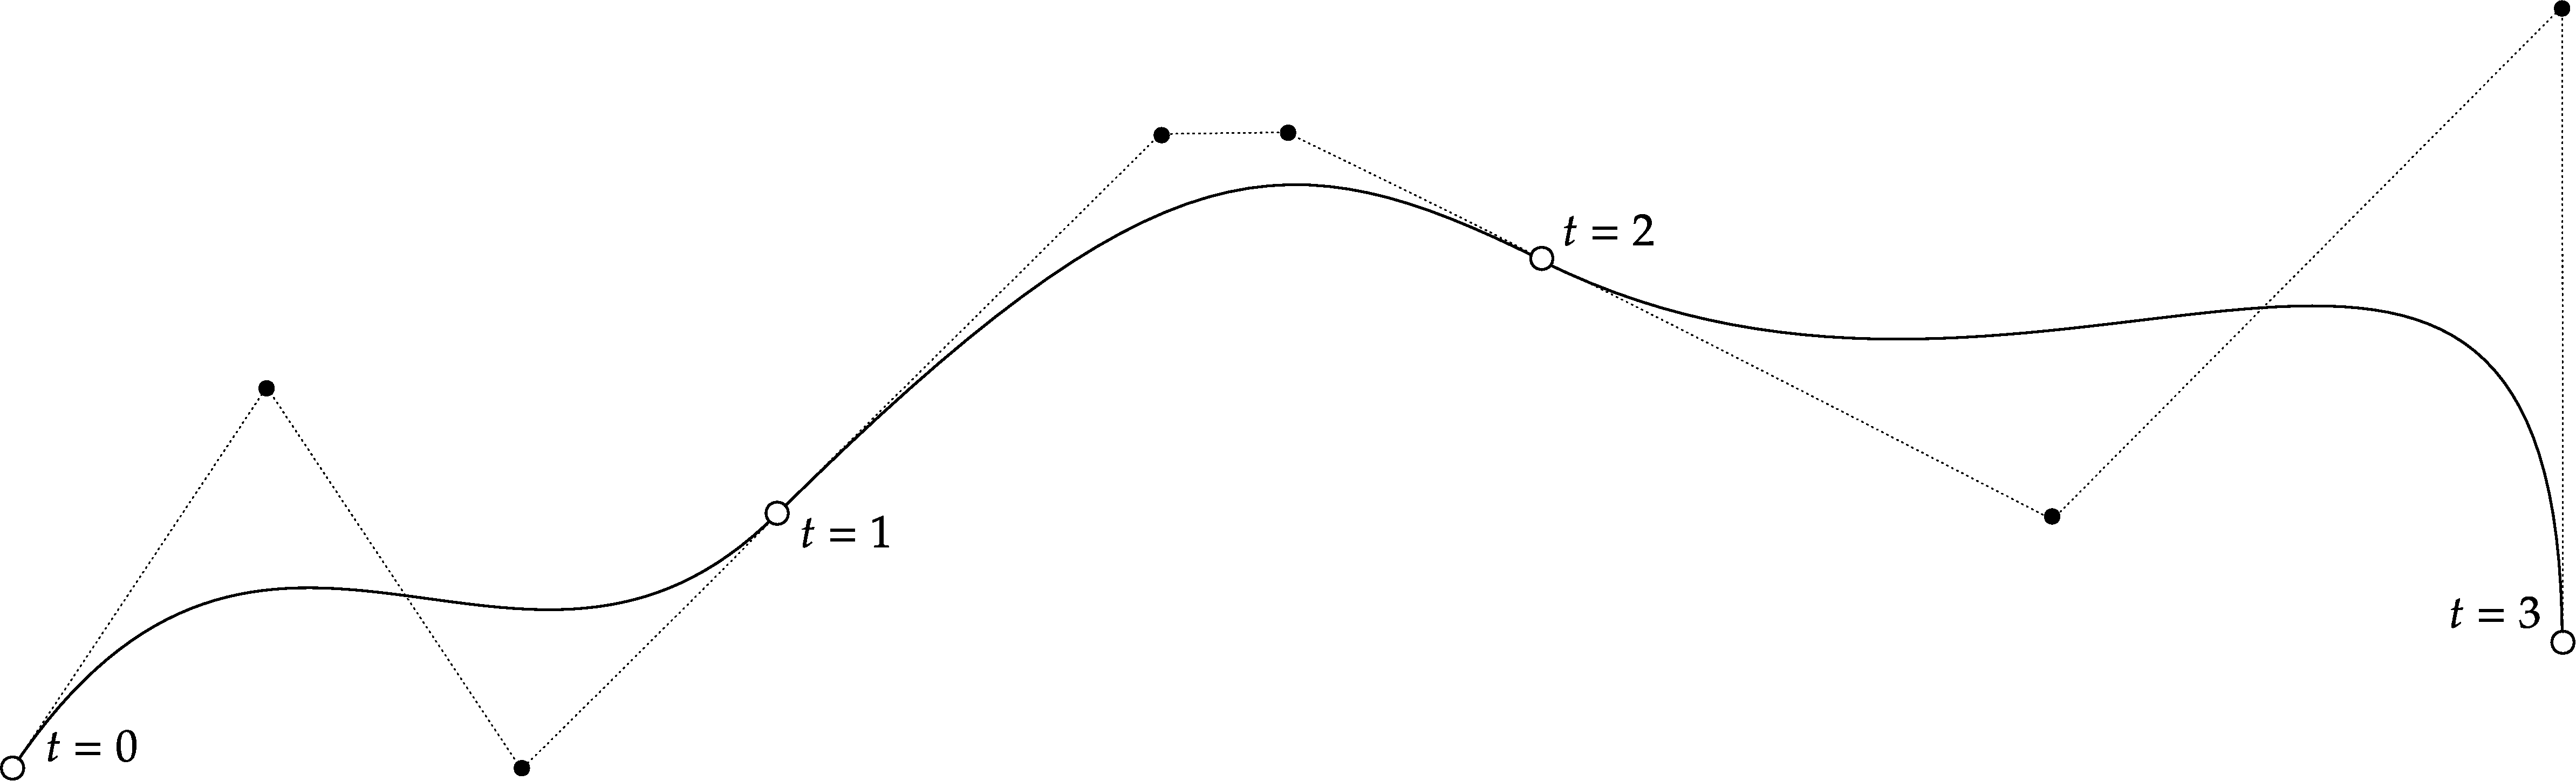
\includegraphics[width=\linewidth]{figs/segments}
\caption{A composite B\'ezier curve made from three segments.}%
\label{fig:segments}
\end{figure*}

In a parametric surface \(S(u, v)\), specific values of \(u\) are curves on the surface, as are values of \(v\).
Similarly, a set of two curves with fixed \(u\) and two curves with fixed \(v\) will bound a patch, \eg\ \(S(u, 0)\), \(S(u, 1)\), \(S(0, v)\) and \(S(1, v)\) (Figure~\ref{fig:patch}).

\begin{figure}
\centering
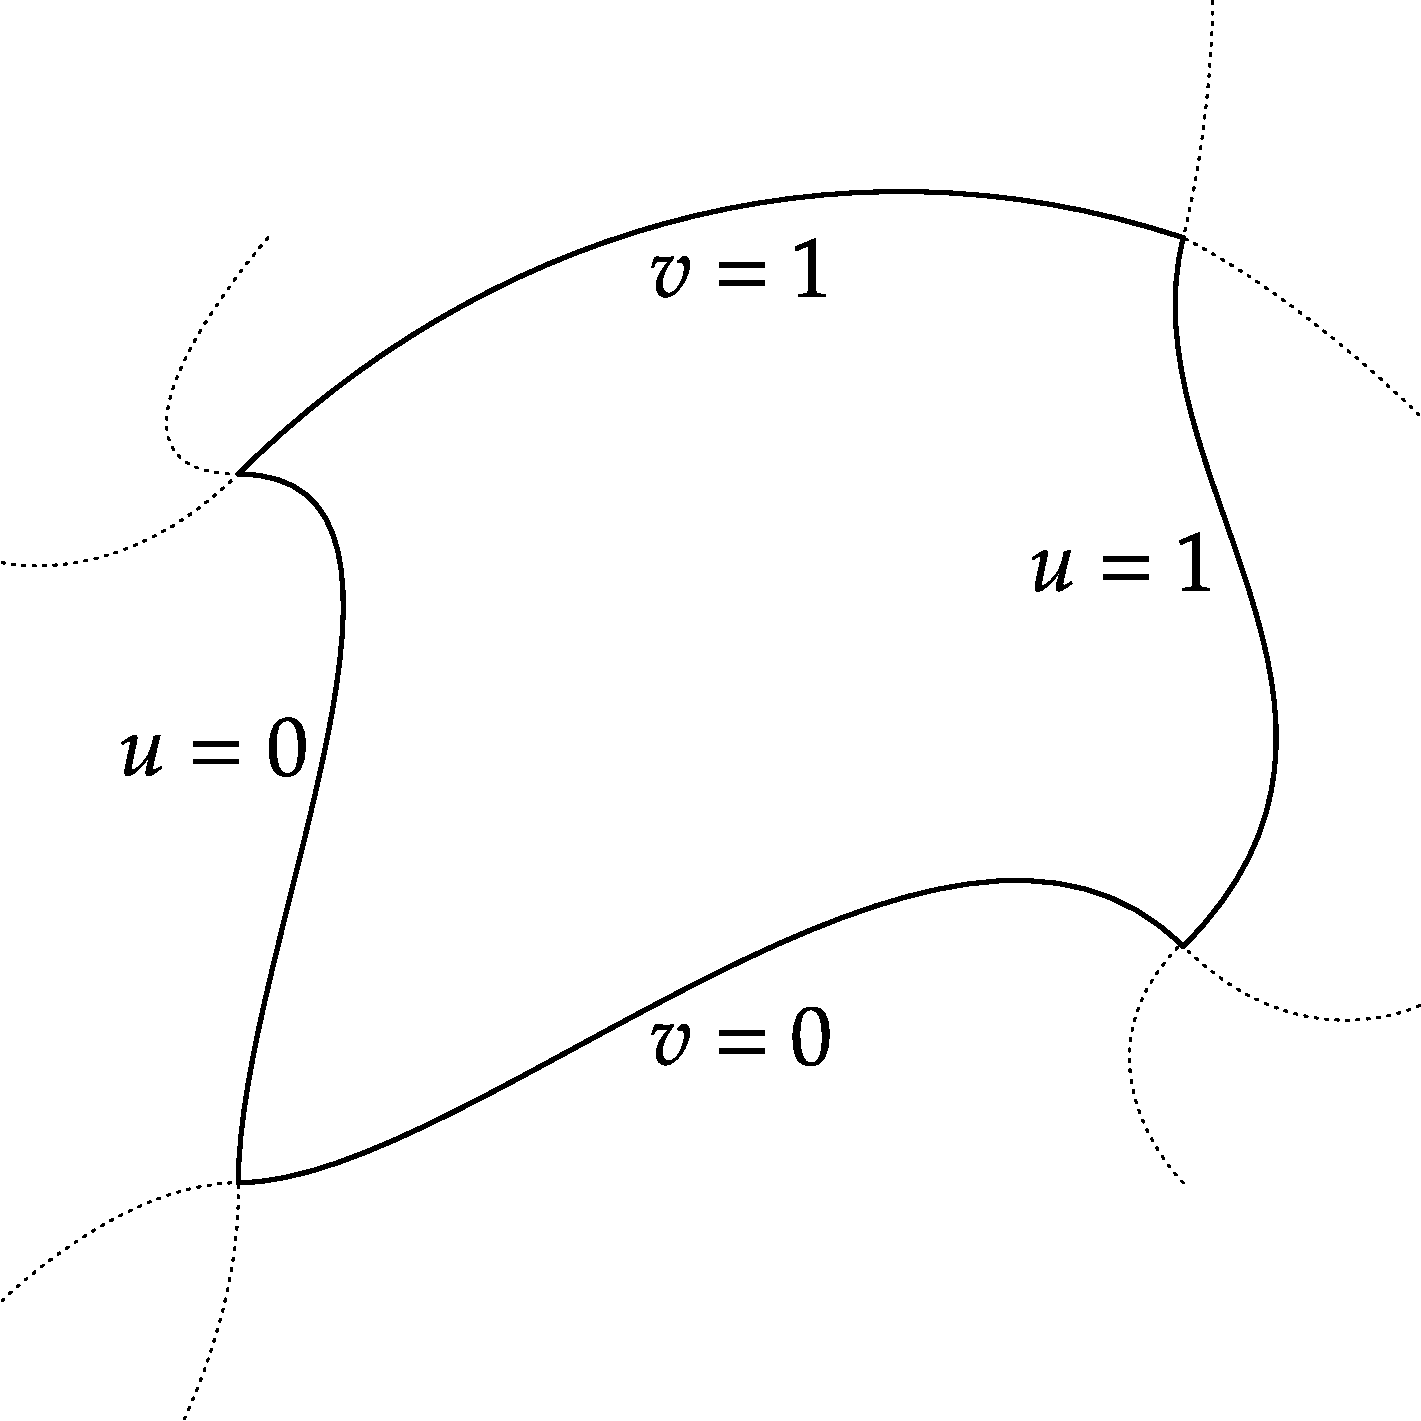
\includegraphics[width=0.5\linewidth]{figs/patch}
\caption{A B\'ezier rectangular patch.}%
\label{fig:patch}
\end{figure}

\subsection{Continuity}

In order to describe how segments/patches should be joined, we rely on the concept of continuity, of which there are two types: geometric and parametric.
Geometric continuity\marginnote{geometric continuity}\index{geometric continuity} can be defined as follows:

\begin{description}
\item[Positional] (\(G^0\)) continuity\marginnote{positional continuity}\index{positional continuity}\marginnote{\(G^0\) continuity}\index{\(G^0\) continuity} means that the boundary of a segment or patch matches that of its neighbours, \ie\ there are no holes at common boundaries (Figure~\ref{subfig:g0});
\item[Tangential] (\(G^1\))\marginnote{tangential continuity}\index{tangential continuity}\marginnote{\(G^1\) continuity}\index{\(G^1\) continuity} means that the angles of segments or patches match those of its neighbours at their common boundaries, \ie\ no sharp edges at common boundaries (Figure~\ref{subfig:g1});
\item[Curvature] (\(G^2\))\marginnote{curvature continuity}\index{curvature continuity}\marginnote{\(G^2\) continuity}\index{\(G^2\) continuity} means that the curvature of a segment or patch match that of its neighbours at their common boundaries, \ie\ no `soft' edges at common boundaries.
\end{description}

\begin{figure}
\centering
\begin{subfigure}{0.4\linewidth}
\includegraphics[width=\linewidth]{figs/g0}
\caption{}%
\label{subfig:g0}
\end{subfigure}%
\begin{subfigure}{0.4\linewidth}
\includegraphics[width=\linewidth]{figs/g1}
\caption{}%
\label{subfig:g1}
\end{subfigure}%
\caption{Continuity: (a) \(G_0\) and (b) \(G_1\). \(G_2\) continuity is difficult to achieve with B\'ezier curves.}%
\label{fig:g}
\end{figure}

Generalising from here, we can say that a curve has \(G^n\) continuity\marginnote{\(G^n\) continuity}\index{\(G^n\) continuity} at a boundary point when the \(n\)-th derivatives have the same direction at that point.
If they have the same magnitude as well, it is also said to have \(C^n\) continuity.
Therefore, \(C^n\) continuity\marginnote{\(C^n\) continuity}\index{\(C^n\) continuity} implies \(G^n\) continuity.

\section{B\'ezier curves}

B\'ezier curves\marginnote{B\'ezier curve}\index{B\'ezier curve} are parametric curves that are based on a polynomial function with one parameter.
They are named after Pierre B\'ezier, who developed them to model the stylised shapes of cars while working at Renault in the 1960s.
Interestingly enough, they were also independently developed by Paul de Casteljau at Citro\"en, likely before B\'ezier, but it appears that he was not allowed to publish them.
However, De Casteljau's algorithm, which is used to evaluate B\'ezier curves, is named after him.

\subsection{A single B\'ezier segment}

Given a sequence of points, the B\'ezier curve starts from the first point and ends at the last point, whereas the intermediate points are treated as control points that `pull' the curve in their direction, but always remaining inside the convex hull of the points.
This is known as a \emph{B\'ezier segment}\marginnote{B\'ezier segment}\index{B\'ezier segment}.

The tangent vector at the first point points to the second point, whereas the tangent vector at the last point points from the next-to-last point to it.
Similar constructions can be made for the higher derivatives, with the \(n\)-th derivative being determined only by \(n+1\) points.

If there are no intermediate points, the result is a linear B\'ezier curve\marginnote{linear B\'ezier curve}\index{linear B\'ezier curve}, which is equivalent to a straight line between the two endpoints.
The most common forms of B\'ezier curves are however quadratic B\'ezier curves\marginnote{quadratic B\'ezier curve}\index{quadratic B\'ezier curve} (Figure~\ref{fig:quadratic}), which have one intermediate point, \eg\ \(p_{\mathrm{quadratic}} = (p_0, p_1, p_2)\), and cubic B\'ezier curves (Figure~\ref{fig:cubic}), which have two intermediate points, \eg\ \(p_{\mathrm{cubic}} = (p_0, p_1, p_2, p_3)\).
Note the tangent vectors in both figures, as well as how the curves always fit within the convex hull of the points.

\begin{figure*}
\centering
\includegraphics[width=\linewidth]{figs/quadratic}
\caption{Three quadratic B\'ezier curves}%
\label{fig:quadratic}
\end{figure*}

\begin{figure*}
\centering
\includegraphics[width=\linewidth]{figs/cubic}
\caption{Three cubic B\'ezier curves}%
\label{fig:cubic}
\end{figure*}

A B\'ezier curve \(C\) can be formulated as a sort of weighted average of its points \((p_i, \ldots, p_n)\):

\begin{equation}
\label{eq:beziercurve}
C(t) = \sum_{i=0}^n B^n_i(t) p_i\text{, for }0 \leq t \leq 1
\end{equation}

where \(B^n_i\) is the weight associated with the point \(p_i\).

Intuitively, you can imagine that we want this weight to reach a maximum when we are close to the point and decrease as we move farther from it.
For example, in a quadratic B\'ezier curve, \(B^n_0\) should start from its maximum value at \(t=0\) and decrease as \(t\) increases, \(B^n_1\) should start low, increase to reach a maximum at \(t=0.5\) and decrease afterwards, and \(B^n_2\) should start from its lowest point and increase to reach its maximum at \(t=1\).

The exact functions used to determine the weights in B\'ezier curves are called \emph{Bernstein polynomials}\marginnote{Bernstein polynomials}\index{Bernstein polynomials} (Figure~\ref{fig:bernstein}), named after Sergei Natanovich Bernstein who discovered them in the 1910s.
These are given by:

\begin{equation}
\label{eq:bernstein}
B^n_i(t) = \binom{n}{i} t^i (1-t)^{n-i}\text{, where }\binom{n}{i} = \frac{n!}{i! (n-i)!}
\end{equation}

where \(n\) is the degree of the B\'ezier curve, \ie\ 1 for linear, 2 for quadratic, 3 for cubic, etc.
\(\binom{n}{i}\) is the \emph{binomial coefficient}\marginnote{binomial coefficient}\index{binomial coefficient}, which is equivalent to the \(i\)-th column of the \(n\)-th row in Pascal's triangle\marginnote{Pascal's triangle}\index{Pascal's triangle} (Figure~\ref{fig:pascal}).

\begin{figure*}
\centering
\begin{subfigure}{0.5\linewidth}
\includegraphics[width=\linewidth]{figs/bernstein1}
\caption{}%
\label{subfig:bernstein1}
\end{subfigure}%
\begin{subfigure}{0.5\linewidth}
\includegraphics[width=\linewidth]{figs/bernstein2}
\caption{}%
\label{subfig:bernstein2}
\end{subfigure}\\
\begin{subfigure}{0.5\linewidth}
\includegraphics[width=\linewidth]{figs/bernstein3}
\caption{}%
\label{subfig:bernstein3}
\end{subfigure}%
\caption{Weights obtained from the Bernstein polynomials for (a) linear, (b) quadratic and (c) cubic B\'ezier curves.}%
\label{fig:bernstein}
\end{figure*}

\begin{figure}
\centering
\includegraphics[width=0.4\linewidth]{figs/pascal-triangle}
\caption{Pascal's triangle, where the numbers are obtained by adding the numbers in the row above (starting from a single 1).}%
\label{fig:pascal}
\end{figure}

Linear B\'ezier curves (\(n = 1\)) are thus given by:

\begin{align}
\label{eq:bezier1}
C(t) &= \sum_{i=0}^1 B^1_i(t) p_i \nonumber \\
&= (1-t) p_0 + t p_1\text{, for }0 \leq t \leq 1.
\end{align}

which is equivalent to the parametric equation of the line we discussed in the background.
Quadratic B\'ezier curves (\(n = 2\)) are given by:

\begin{align}
\label{eq:bezier2}
C(t) &= \sum_{i=0}^2 B^2_i(t) p_i \nonumber \\
&= (1-t)^2 p_0 + 2 t (1-t) p_1 + t^2 p_2\text{, for }0 \leq t \leq 1.
\end{align}

And cubic B\'ezier curves (\(n = 3\)) are given by:

\begin{small}
\begin{align}
\label{eq:bezier3}
C(t) &= \sum_{i=0}^3 B^3_i(t) p_i \nonumber \\
&= (1-t)^3 p_0 + 3 t (1-t)^2 p_1 + 3 t^2 (1-t) p_2 + t^3 p_3\text{, for }0 \leq t \leq 1.
\end{align}
\end{small}

\subsection{Composite B\'ezier curves}

Now, let us discuss how to join multiple B\'ezier segments together smoothly into a \emph{composite B\'ezier curve}\marginnote{composite B\'ezier curve}\index{composite B\'ezier curve} or a \emph{polybezier}\marginnote{polybezier}\index{polybezier} (accent usually omitted).
When they are joined in a loop, \ie\ joining the last to the first, it is sometimes called a \emph{beziergon}\marginnote{beziergon}\index{beziergon} or \emph{bezigon}\marginnote{bezigon}\index{bezigon}.
Many common vector file formats use these, including several font formats, PDF files, and SVG images.
Figure~\ref{fig:pointtypes} also shows how these commonly look in software, where the intermediate control points are shown as `handles' around the data points.

As we mentioned before, high-degree polynomials are undesirable because they tend to wobble and are hard to control.
It is therefore usually better to create composite B\'ezier curves by connecting B\'ezier segments made from low-degree B\'ezier curves using only a few control points, most often cubics.

Connecting multiple B\'ezier segments with \(G_0\) or \(C_0\) continuity simply means that their common endpoint should be the same.
That is, if we have a composite B\'ezier curve formed by two adjacent B\'ezier segments, where the first is defined by the points \((p_0, \ldots, p_n)\) and the second is defined by the points \((q_0, \ldots, q_n)\), we need to enforce that \(p_n = q_0\).

As we previously discussed, the tangent vector of the endpoint of a B\'ezier curve is related only to the endpoint and its neighbour.
Therefore, \(G_1\) continuity can be achieved by making sure that the common endpoint and its two neighbours, \ie\ \(p_{n-1}\) and \(q_1\), are collinear (Figure~\ref{fig:polybezier}).
For \(C_1\) continuity, they should also be evenly spaced.
\(G_2\) and \(C_2\) continuity is hard to achieve, so we will not discuss it here.

\begin{figure}
\centering
\begin{subfigure}{0.5\linewidth}
\includegraphics[width=\linewidth]{figs/polybezierg}
\caption{}%
\label{subfig:polybezierg}
\end{subfigure}%
\begin{subfigure}{0.5\linewidth}
\includegraphics[width=\linewidth]{figs/polybezierc}
\caption{}%
\label{subfig:polybezierc}
\end{subfigure}%
\caption{Two composite B\'ezier curves with: (a)\(G_1\) continuity and (b) \(C_1\) continuity (bottom).}%
\label{fig:polybezier}
\end{figure}

\section{B\'ezier surfaces}
\subsection{Rectangular B\'ezier surfaces}

Moving on to 3D, the most common implementation of B\'ezier surfaces uses rectangular patches, which are made of grids of points.
The most common are biquadratic\marginnote{biquadratic B\'ezier surface}\index{biquadratic B\'ezier surface} (\(3 \times 3\); Figure~\ref{fig:quadraticsurf}) and bicubic\marginnote{bicubic B\'ezier surface}\index{bicubic B\'ezier surface} (\(4 \times 4\); Figure~\ref{fig:cubicsurf}) surfaces, which are defined based on square matrices of points, such as:

\begin{figure}
\centering
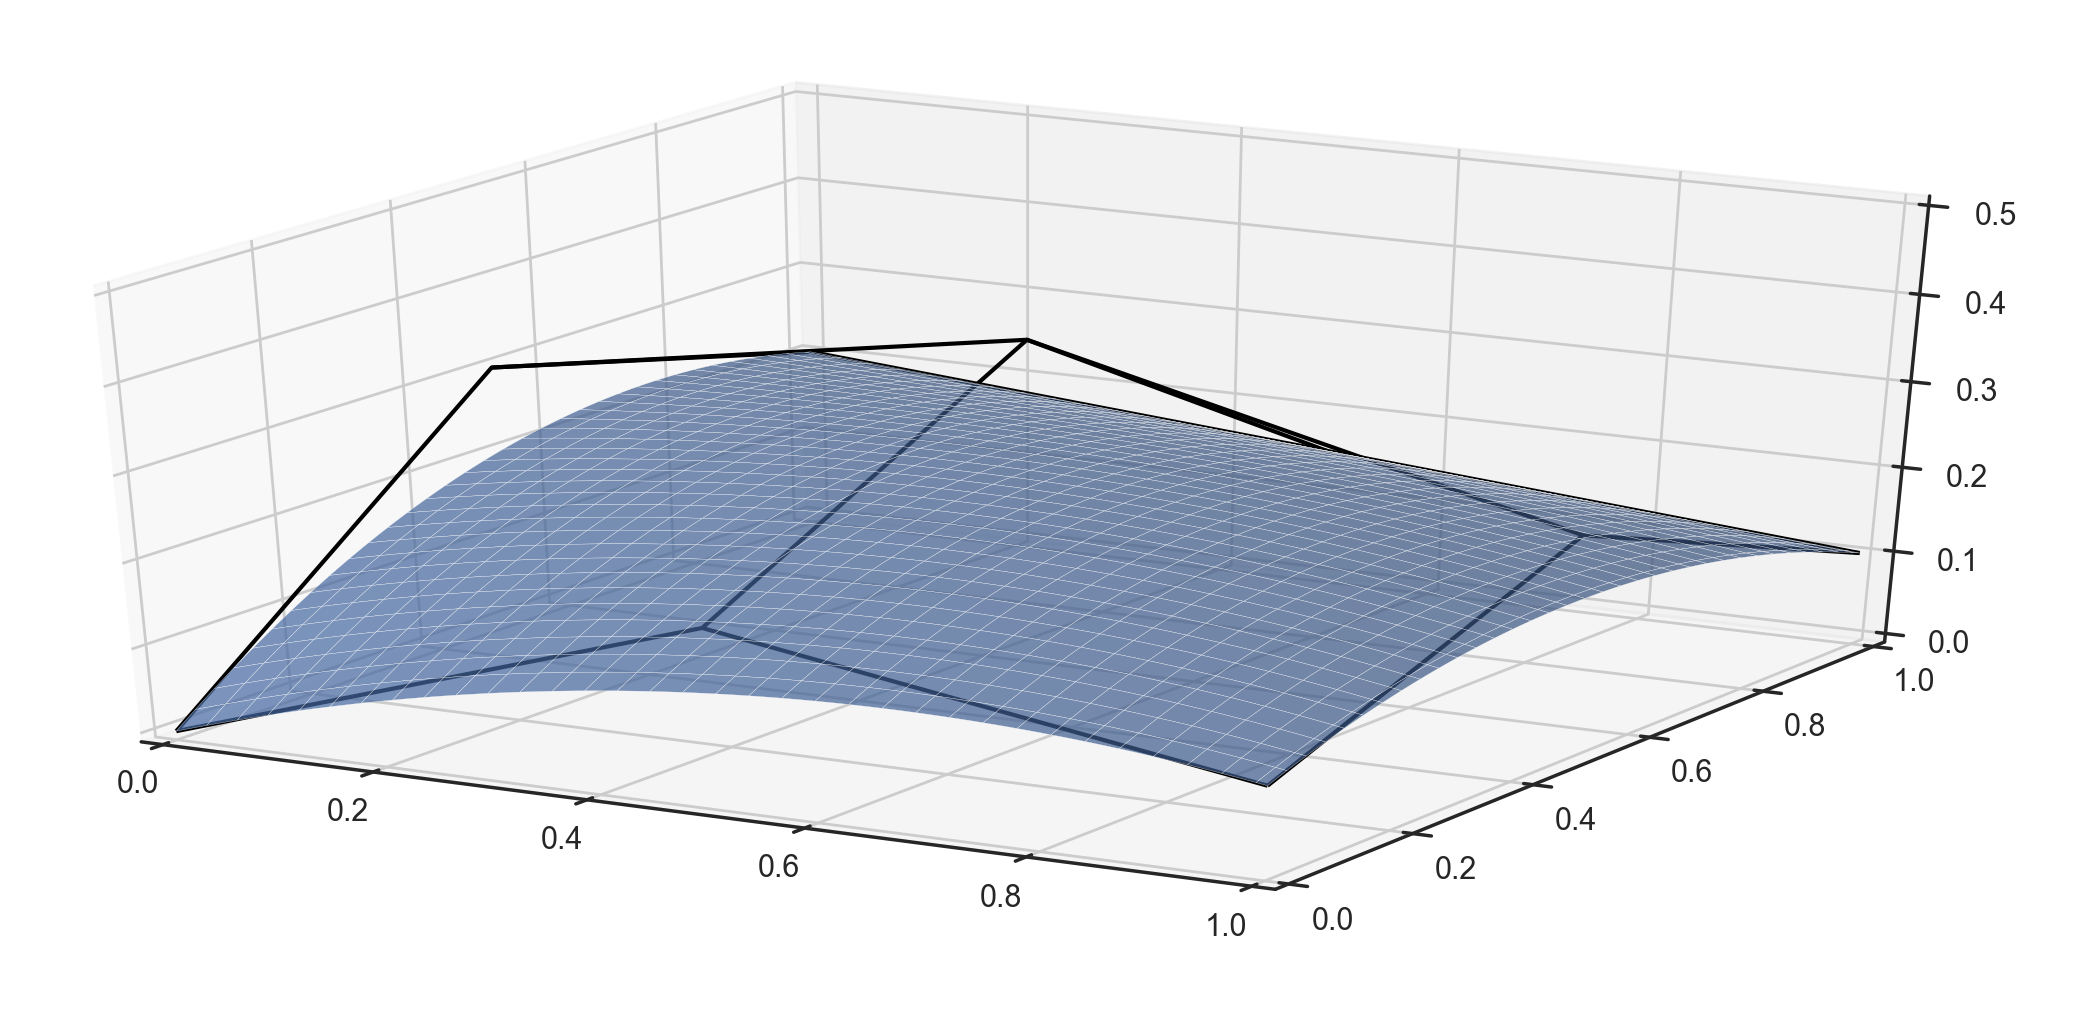
\includegraphics[width=\linewidth]{figs/quadraticsurf}
\caption{A B\'ezier biquadratic surface and the points that define it.
Note how the four corners are the only data points and how the surface is tangent to them.}%
\label{fig:quadraticsurf}
\end{figure}

\begin{figure}
\centering
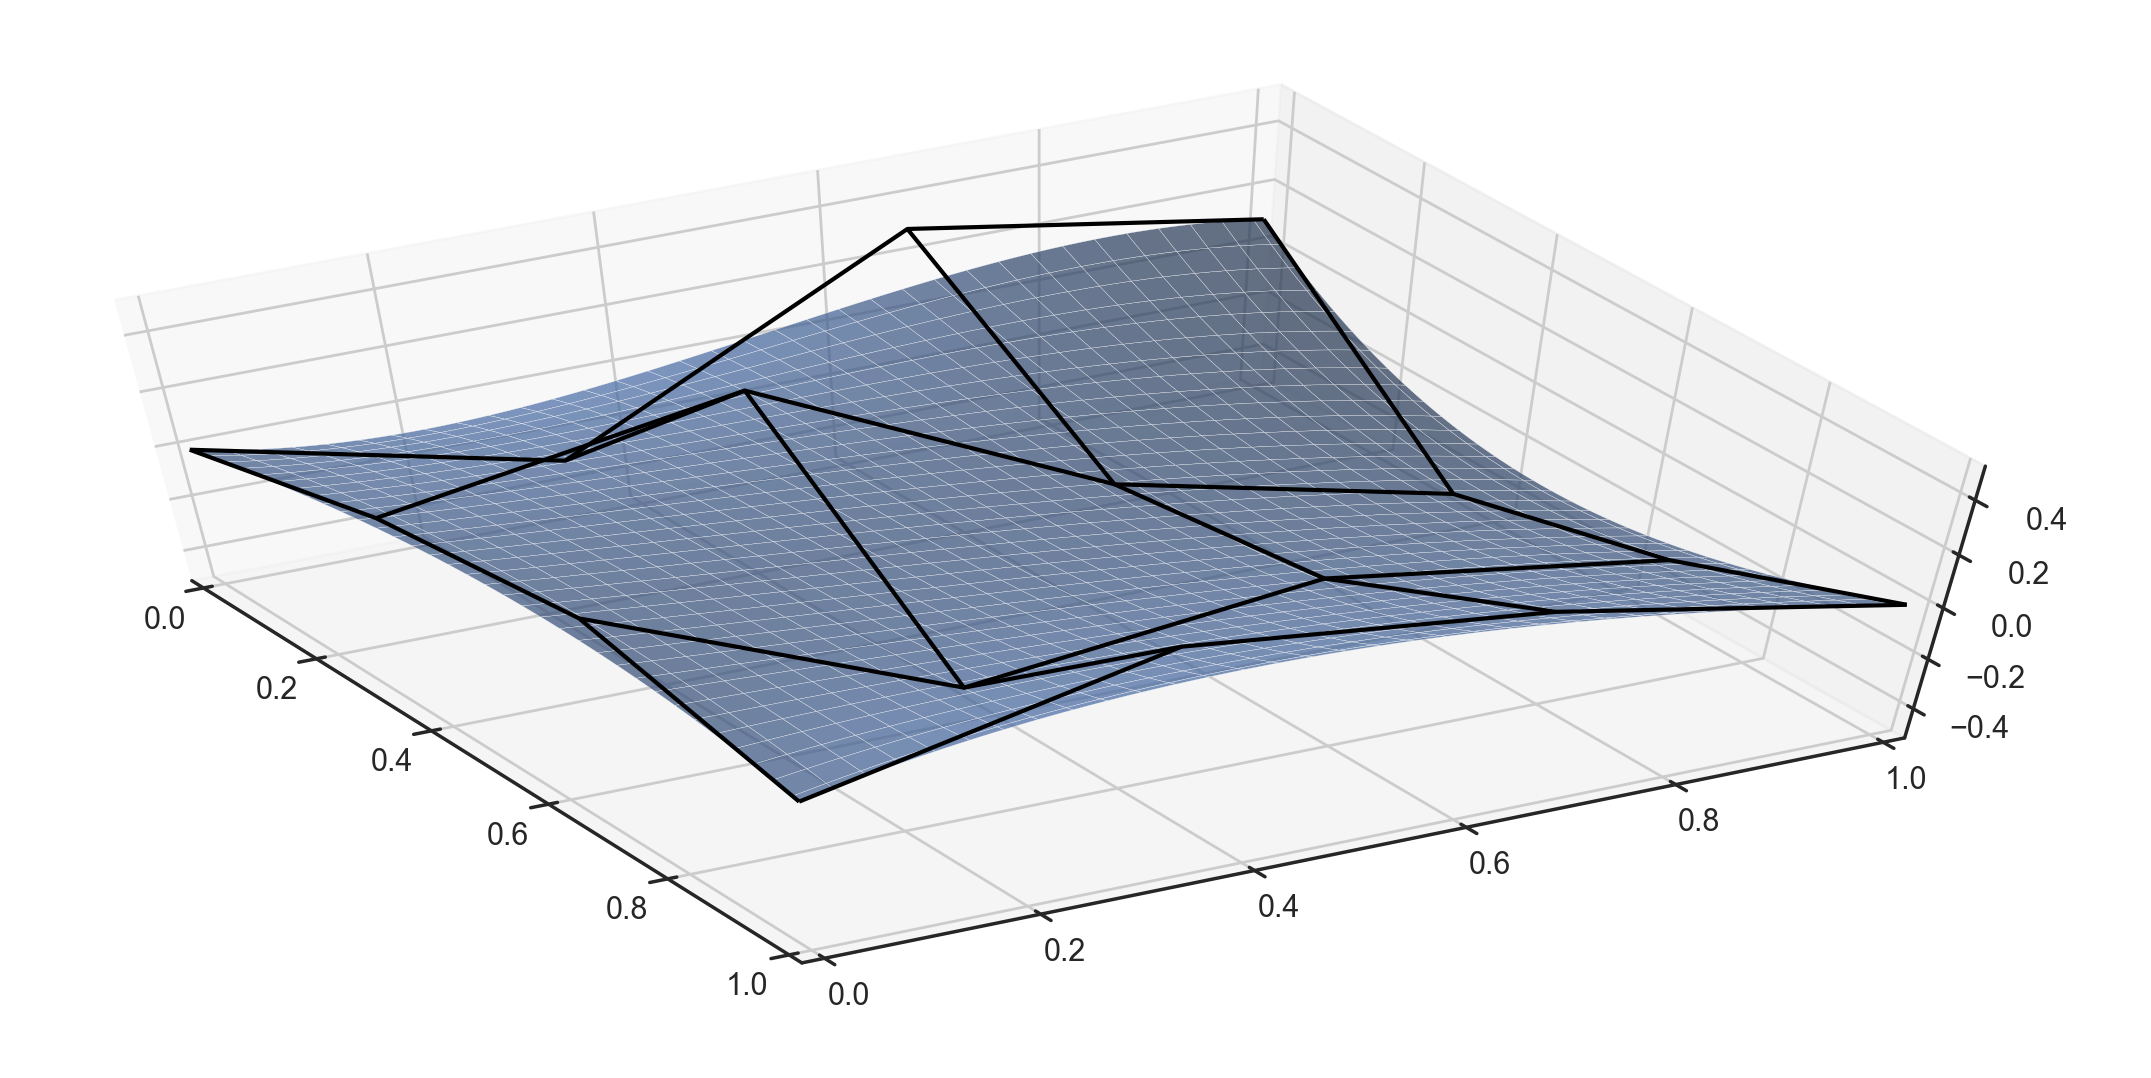
\includegraphics[width=\linewidth]{figs/cubicsurf}
\caption{A B\'ezier bicubic surface and the points that define it.
Note how the four corners are the only data points and how the surface is tangent to them.}%
\label{fig:cubicsurf}
\end{figure}

\begin{align}
p_{\mathrm{biquadratic}} &= \left(\begin{array}{ccc}
p_{0,0} & p_{0,1} & p_{0,2} \\
p_{1,0} & p_{1,1} & p_{1,2} \\
p_{2,0} & p_{2,1} & p_{2,2} 
\end{array}\right)\text{, and } \\
p_{\mathrm{bicubic}} &= \left(\begin{array}{cccc}
p_{0,0} & p_{0,1} & p_{0,2} & p_{0,3} \\
p_{1,0} & p_{1,1} & p_{1,2} & p_{1,3} \\
p_{2,0} & p_{2,1} & p_{2,2} & p_{2,3} \\
p_{3,0} & p_{3,1} & p_{3,2} & p_{3,3}
\end{array}\right),
\end{align}

where only the four corner points are data points and all the others are control points.
Note that the four sides of a B\'ezier surface are B\'ezier curves using the points on the top/bottom/left/right of the matrix.

A rectangular B\'ezier surface is described as:

\begin{equation}
\label{eq:bezierrectangle}
S(u, v) = \sum_{i=0}^n \sum_{j=0}^m B^n_i(u) B^m_j(v) p_{i,j}\text{, for }0 \leq u \leq 1, 0 \leq v \leq 1.
\end{equation}

where \(p_{i,j}\) is a point in an \(m \times n\) matrix that defines the data points and control points used for the patch.

As with composite B\'ezier curves, \emph{composite B\'ezier surfaces}\marginnote{composite B\'ezier surface}\index{composite B\'ezier surface} can be created by joining together multiple rectangular B\'ezier patches\marginnote{B\'ezier patch}\index{B\'ezier patch}.
These follow the same logic as the composite B\'ezier curves.

In order to get \(G_0\) and \(C_0\) continuity, the common points at the boundary of the two matrices should be the same.
That is, if we have a composite B\'ezier surface formed by two adjacent B\'ezier rectangular patches, where the first is defined by the matrix \(p\) and the second by the matrix \(q\), which are defined as:

\begin{equation}
p = \left(\begin{array}{ccc}
p_{0,0} & \cdots & p_{0,n} \\
\vdots & \ddots & \vdots \\
p_{m,0} & \cdots & p_{m,n} 
\end{array}\right),
q = \left(\begin{array}{ccc}
q_{0,0} & \cdots & q_{0,n} \\
\vdots & \ddots & \vdots \\
q_{m,0} & \cdots & q_{m,n} 
\end{array}\right),
\end{equation}

and they are joined at the curve defined by \(p_{i,n}\) and \(q_{i,0}\), for \(0 \leq i \leq n\), we simply need to enforce that \(p_{i,n} = q_{i, 0}\).

For \(G_1\) continuity, we need to ensure that the tangent vector at the common curve has the same direction, which is given by:

\begin{equation}
\left. \frac{\partial p(u,v)}{\partial v} \right|_{v=1} = a \left. \frac{\partial q(u,v)}{\partial v} \right|_{v=0}.
\end{equation}

where \(a\) can have any positive value.
For \(C_1\) continuity, the magnitude of the vector needs to be the same, which means that \(a = 1\) in the previous equation.
Just as with composite B\'ezier curves, these conditions are achieved when each point along the common boundary curve and its neighbours on either side patch.
That is, for all \(i\), \(p_{i, n-1}\), \(q_{i, 0}\) and \(q_{i, 1}\), are collinear (for \(G_1\)) and also evenly spaced (for \(C_1\)). 

\subsection{Triangular B\'ezier surfaces}

Triangular B\'ezier surfaces\marginnote{triangular B\'ezier surface}\index{triangular B\'ezier surface}, or simply B\'ezier triangles\marginnote{B\'ezier triangle}\index{B\'ezier triangle}, are the other common type of B\'ezier surface.
These are better parametrised in terms of three barycentric coordinates, which we here denote as \(u\), \(v\) and \(w\) (Figure~\ref{fig:triangle}).
Note however that the three coordinates not linearly independent, as they always add up to one.

Triangular B\'ezier surfaces are defined based on triangular arrangements of points of the form:

\begin{figure}
\centering
\begin{subfigure}{0.5\linewidth}
\includegraphics[width=\linewidth]{figs/triangle1}
\caption{}%
\label{subfig:triangle1}
\end{subfigure}%
\begin{subfigure}{0.5\linewidth}
\includegraphics[width=\linewidth]{figs/triangle2}
\caption{}%
\label{subfig:triangle2}
\end{subfigure}%
\caption{The barycentric coordinates used to parametrise triangular B\'ezier surfaces}%
\label{fig:triangle}
\end{figure}

\begin{figure}
\centering
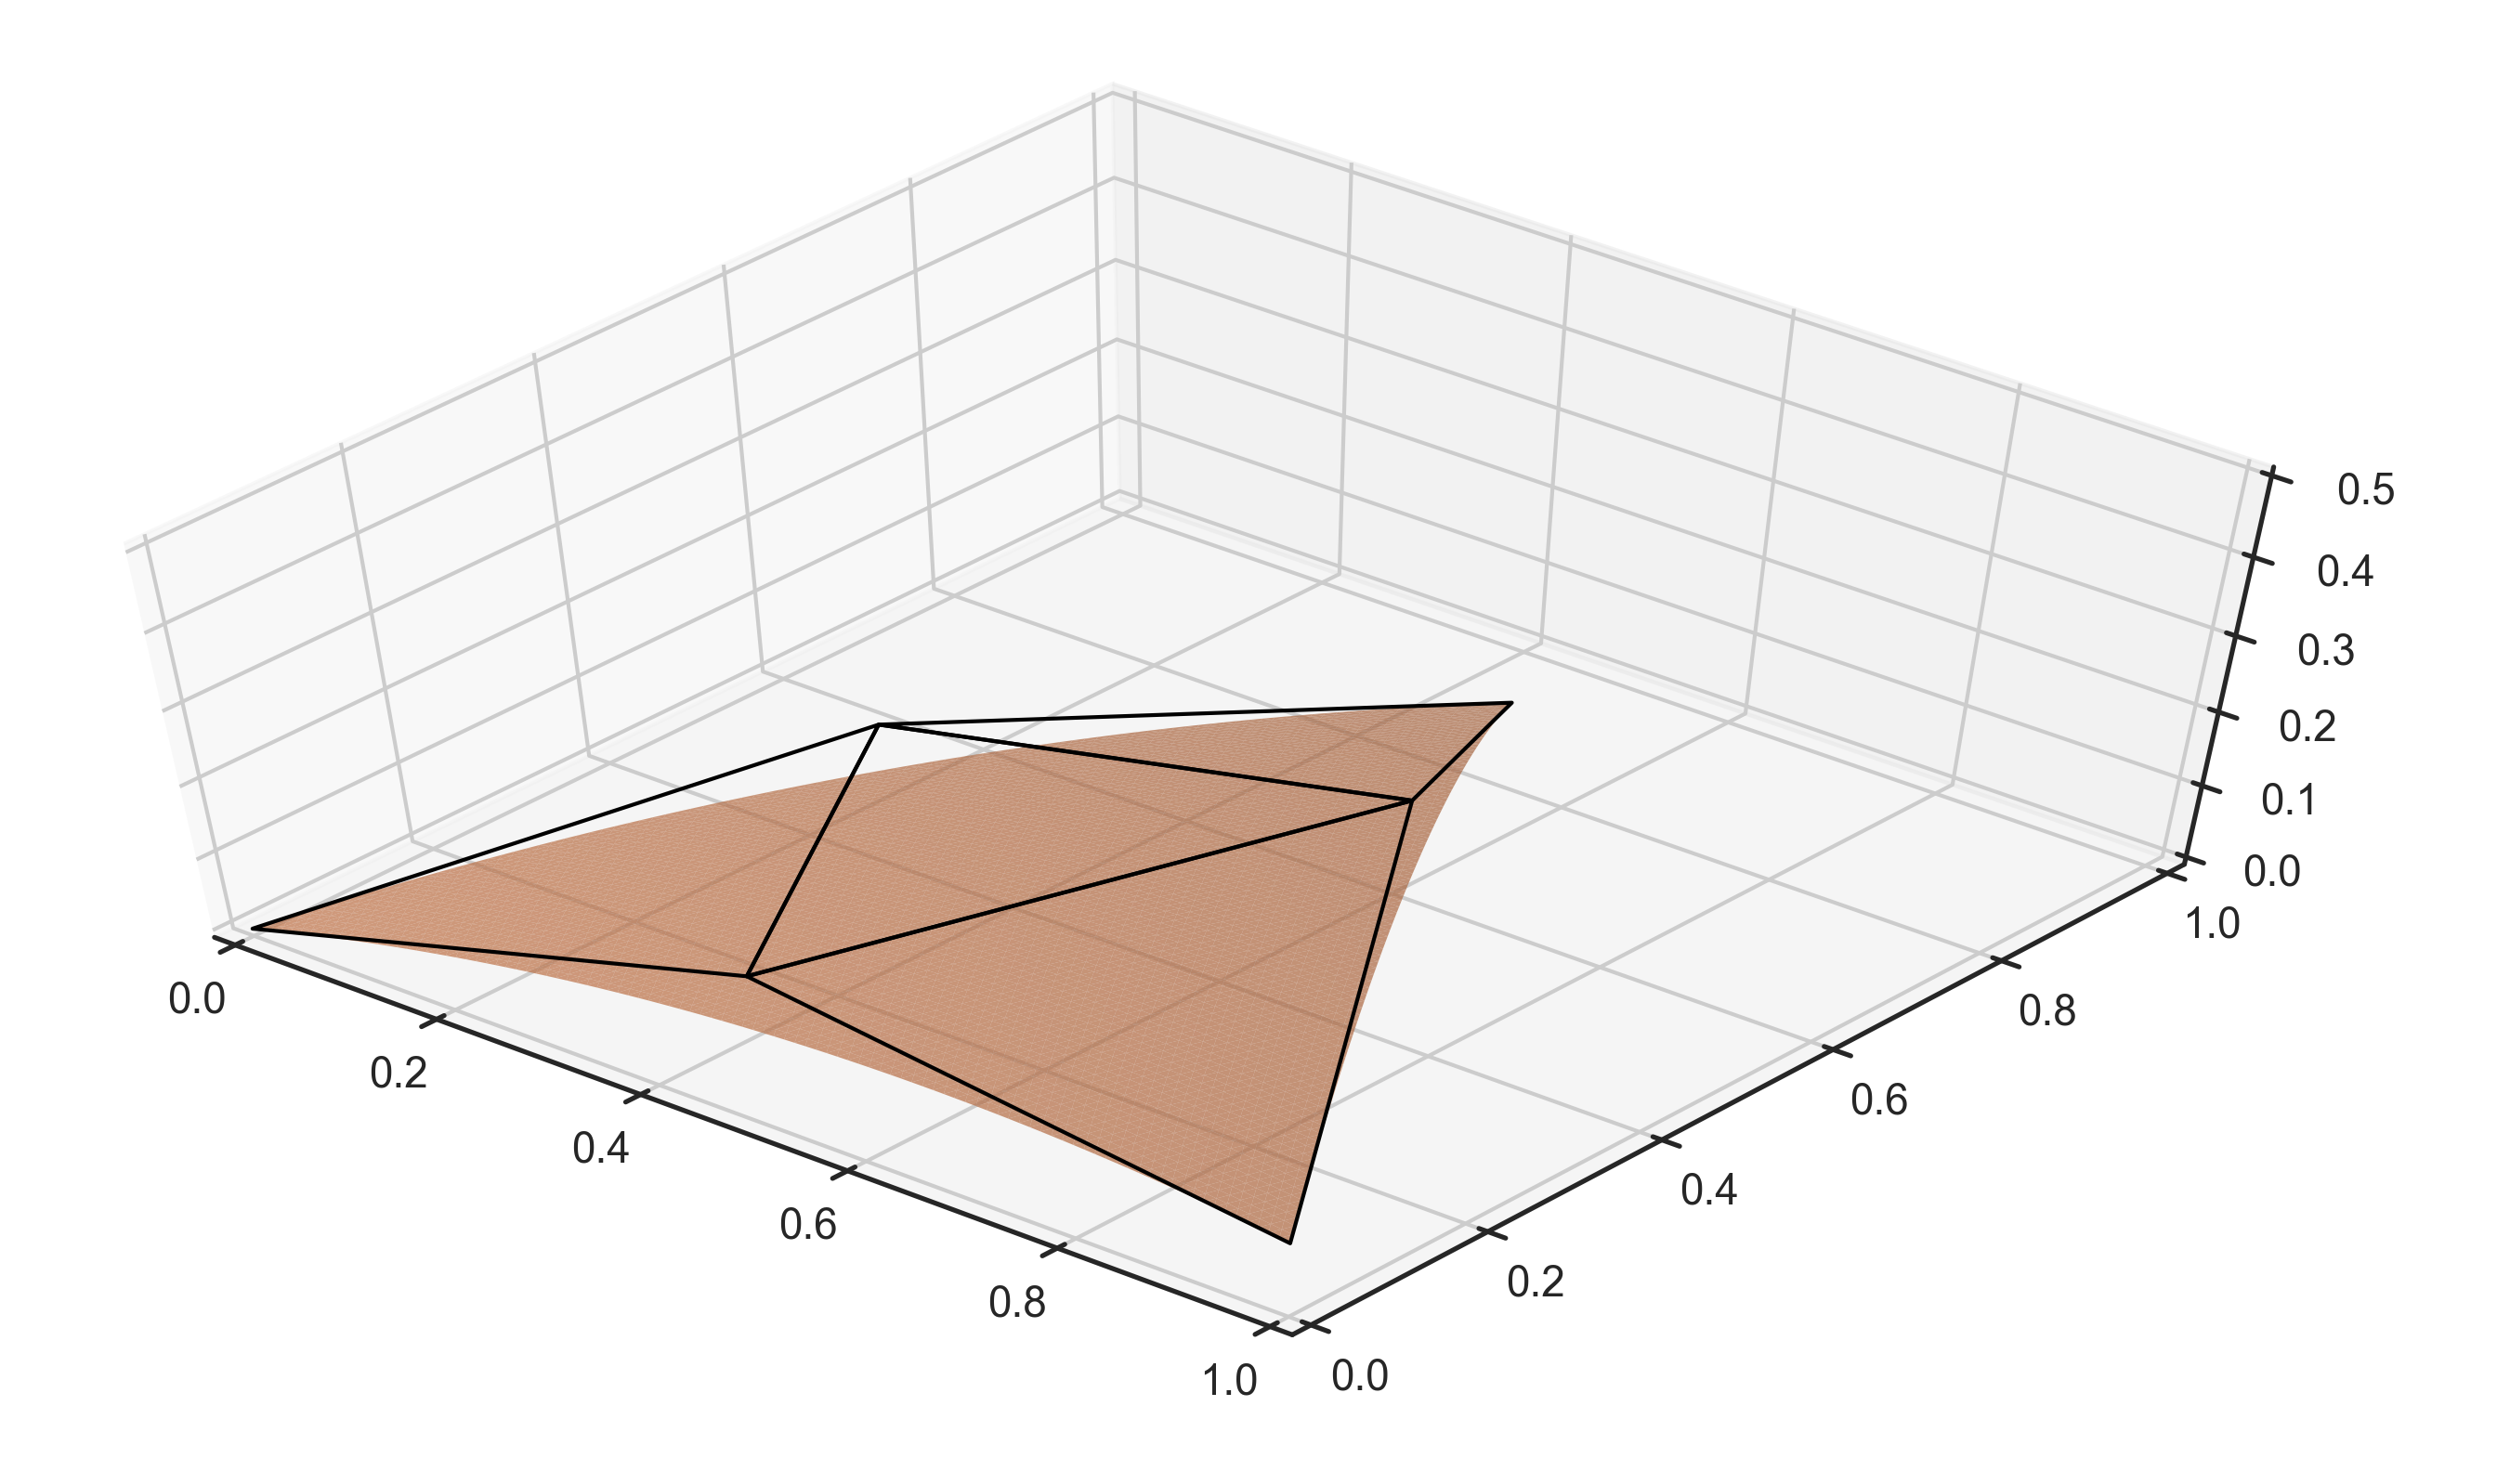
\includegraphics[width=\linewidth]{figs/quadratictri}
\caption{A B\'ezier quadratic triangle and the points that define it.
Note how the three corners are the only data points and how the triangle is tangent to them.}%
\label{fig:quadratictri}
\end{figure}

\begin{figure}
\centering
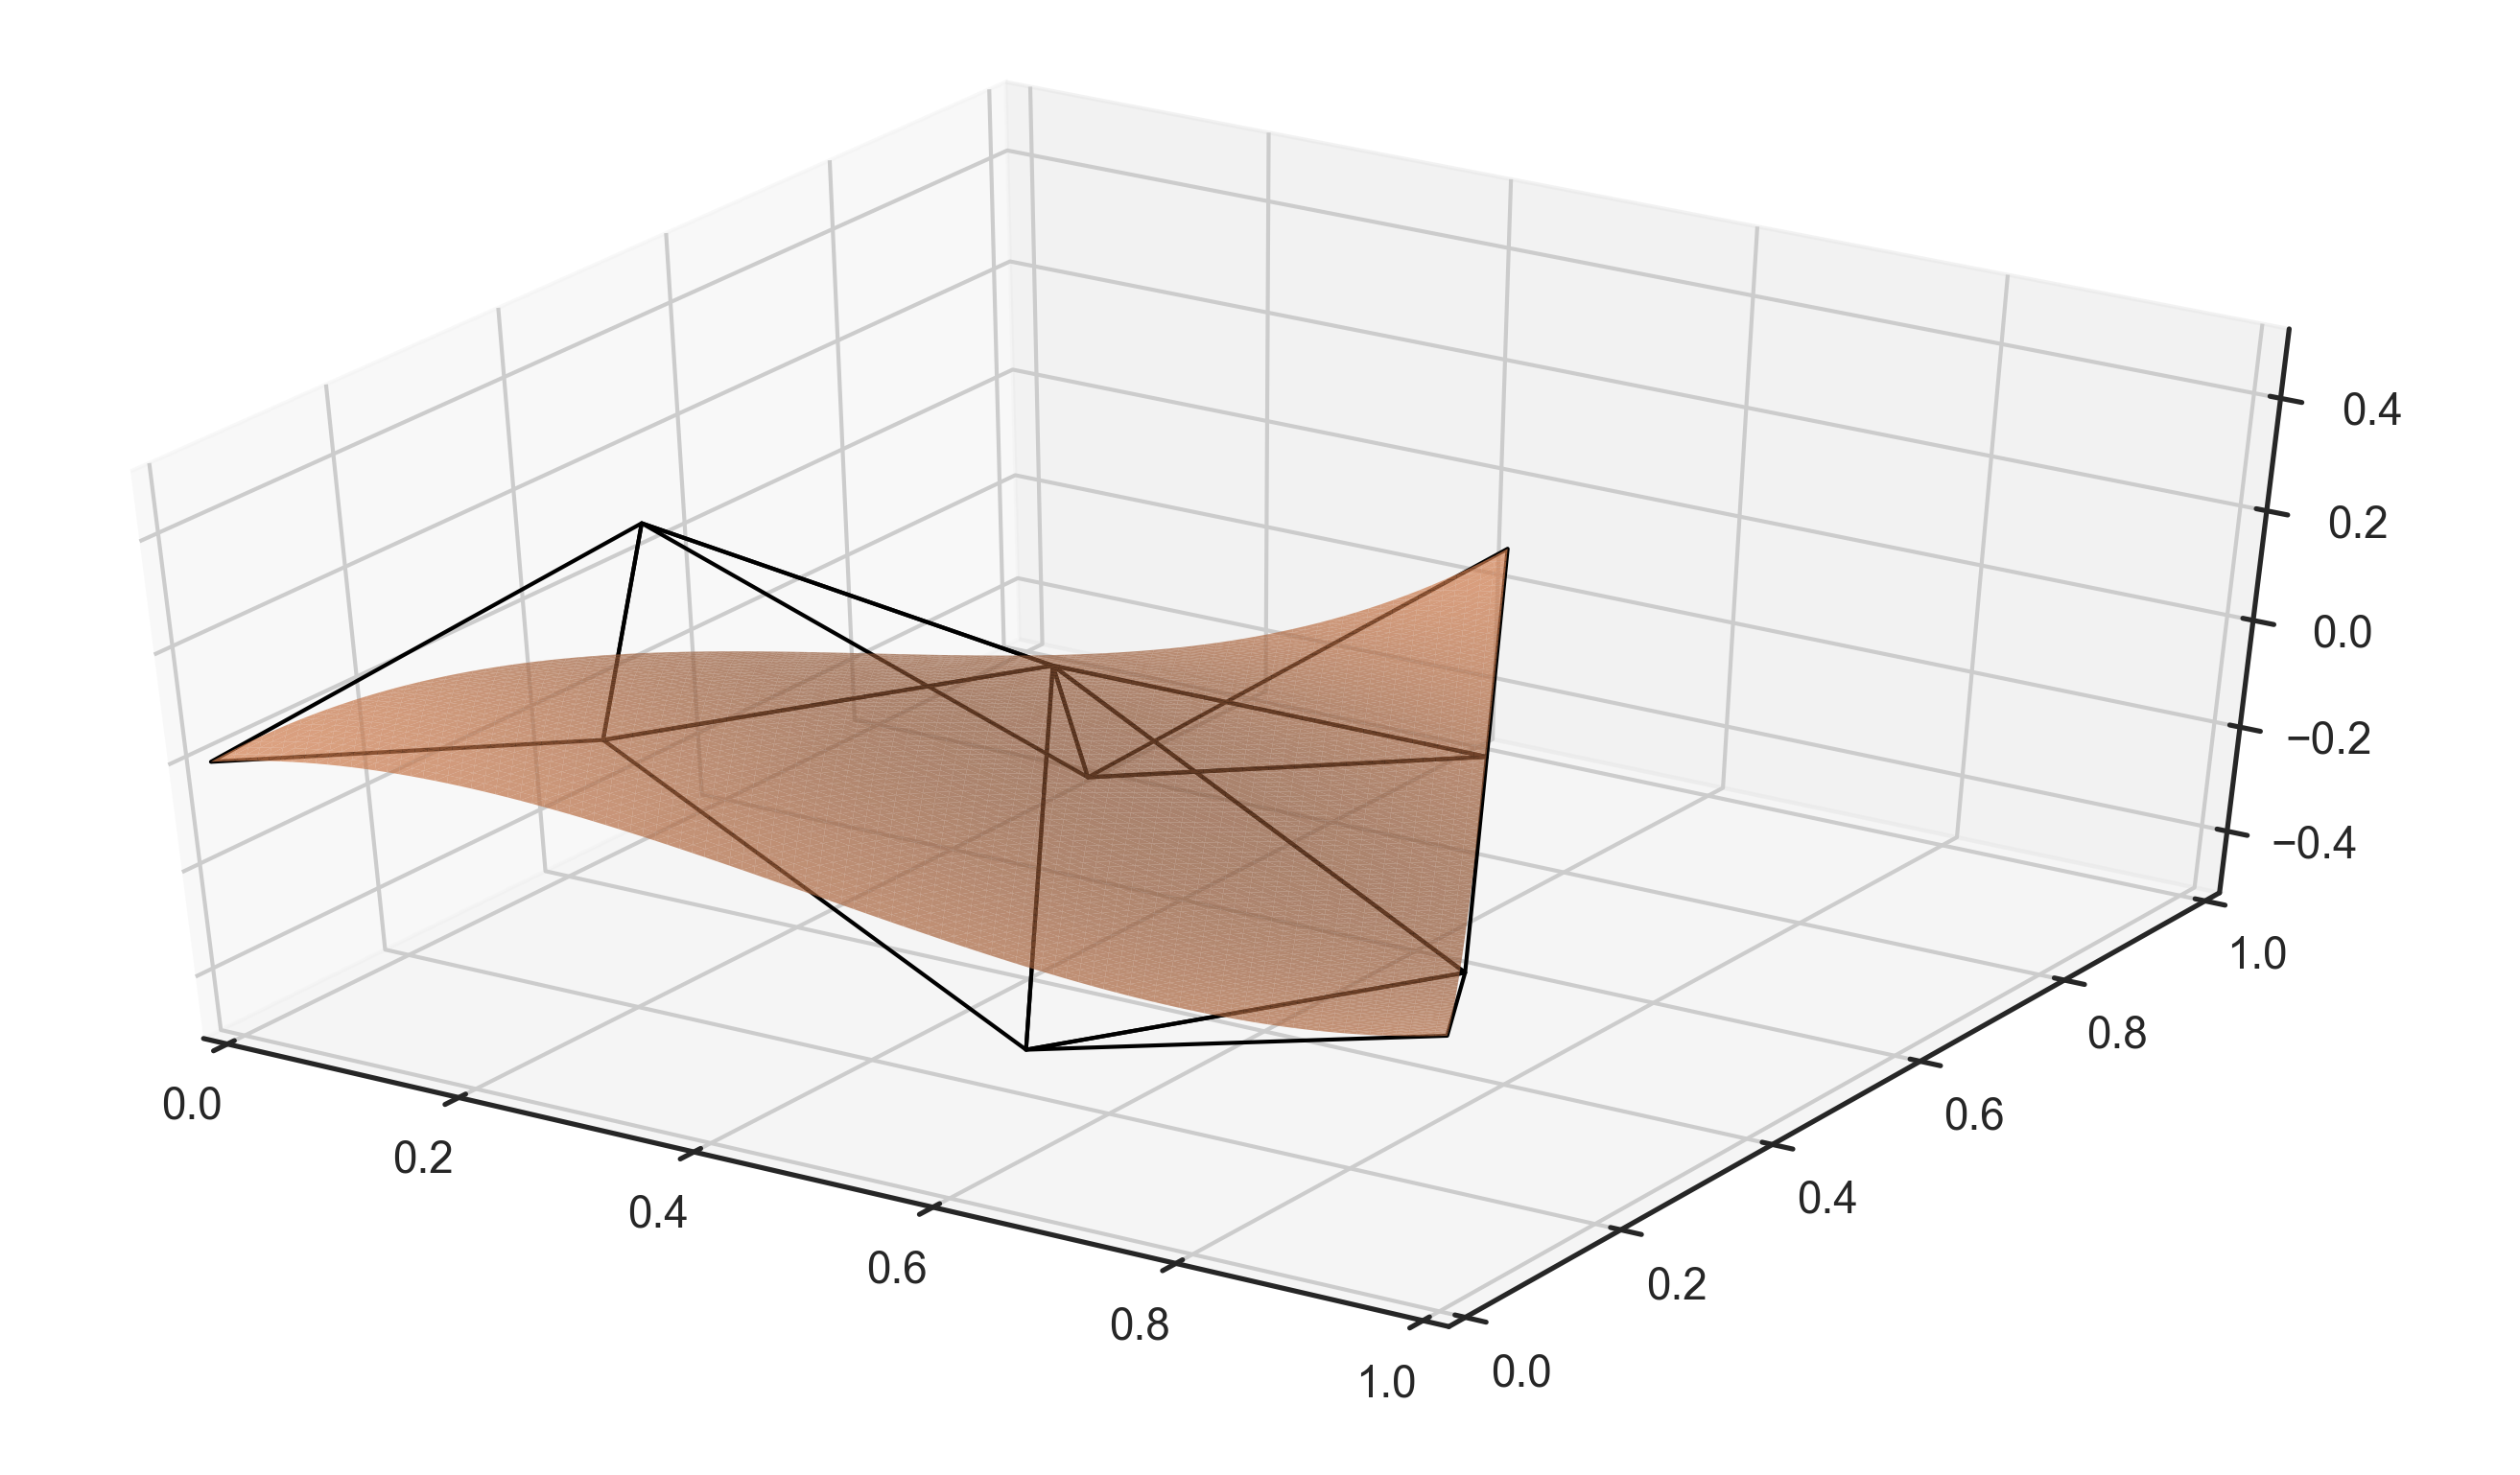
\includegraphics[width=\linewidth]{figs/cubictri}
\caption{A B\'ezier cubic triangle and the points that define it.
Note how the three corners are the only data points and how the triangle is tangent to them.}%
\label{fig:cubictri}
\end{figure}

\begin{align}
p_{\mathrm{linear}} &= \begin{array}{cccc}
& \multicolumn{2}{c}{p_{0,1,0}} & \\
\multicolumn{2}{c}{p_{0,0,1}} & \multicolumn{2}{c}{p_{1,0,0}}
\end{array},\\
p_{\mathrm{quadratic}} &= \begin{array}{cccccc}
\multicolumn{6}{c}{p_{0,2,0}} \\
& \multicolumn{2}{c}{p_{0,1,1}} & \multicolumn{2}{c}{p_{1,1,0}} & \\
\multicolumn{2}{c}{p_{0,0,2}} & \multicolumn{2}{c}{p_{1,0,1}} & \multicolumn{2}{c}{p_{2,0,0}}
\end{array},\\
p_{\mathrm{cubic}} &= \begin{array}{cccccccc}
\multicolumn{8}{c}{p_{0,3,0}} \\
&& \multicolumn{2}{c}{p_{0,2,1}} & \multicolumn{2}{c}{p_{1,2,0}} && \\
& \multicolumn{2}{c}{p_{0,1,2}} & \multicolumn{2}{c}{p_{1,1,1}} & \multicolumn{2}{c}{p_{2,1,0}} & \\
\multicolumn{2}{c}{p_{0,0,3}} & \multicolumn{2}{c}{p_{1,0,2}} & \multicolumn{2}{c}{p_{2,0,1}} & \multicolumn{2}{c}{p_{3,0,0}}
\end{array},
\end{align}

where the surface is described by:

\begin{equation}
S(u,v,w) = \sum_{i+j+k=n \atop i,j,k \geq 0} B^n_{i,j,k}(u,v,w) p_{i,j,k},
\end{equation}

and \(B^n_{i,j,k}\) are the \emph{bivariate Bernstein polynomials}\marginnote{bivariate Bernstein polynomials}\index{bivariate Bernstein polynomials}, which are given by:

\begin{equation}
B^n_{i,j,k}(u,v,w) = \frac{n!}{i!j!k!}u^i v^j w^k
\end{equation}

For the first few values of \(n\), these are:

\begin{align}
B^1_{i,j,k} &= \begin{array}{cccc}
& \multicolumn{2}{c}{v} & \\
\multicolumn{2}{c}{w} & \multicolumn{2}{c}{u}
\end{array},\\
B^2_{i,j,k} &= \begin{array}{cccccc}
\multicolumn{6}{c}{v^2} \\
& \multicolumn{2}{c}{2vw} & \multicolumn{2}{c}{2uv} & \\
\multicolumn{2}{c}{w^2} & \multicolumn{2}{c}{2uw} & \multicolumn{2}{c}{u^2}
\end{array},\\
B^3_{i,j,k} &= \begin{array}{cccccccc}
\multicolumn{8}{c}{v^3} \\
&& \multicolumn{2}{c}{3v^2w} & \multicolumn{2}{c}{3uv^2} && \\
& \multicolumn{2}{c}{3vw^2} & \multicolumn{2}{c}{6uvw} & \multicolumn{2}{c}{3u^2v} & \\
\multicolumn{2}{c}{w^3} & \multicolumn{2}{c}{3uw^2} & \multicolumn{2}{c}{3u^2w} & \multicolumn{2}{c}{u^3}
\end{array}
\end{align}

As with rectangular B\'ezier surfaces, the points on any of the three edges of the triangular B\'ezier surface define a B\'ezier curve.

In order to create a composite B\'ezier surface from triangular B\'ezier patches, we need to have similar constraints as before.
For \(G_0\) and \(C_0\) continuity, the common boundary points should be the same.
That is, if we have a composite B\'ezier surface formed by two adjacent B\'ezier triangular patches, where the first is defined by the matrix \(p\) and the second by the matrix \(q\), which are defined as:

\begin{equation}
p = \begin{array}{cccccc}
&&&& \multicolumn{2}{c}{\multirow{2}{*}{\(p_{0,n,0}\)}} \\
&& \multicolumn{2}{c}{\multirow{2}{*}{\reflectbox{\(\ddots \)}}} \\
\multicolumn{2}{c}{\multirow{2}{*}{\(p_{n,0,0}\)}} &&& \multicolumn{2}{c}{\multirow{2}{*}{\(\vdots \)}} \\
&& \multicolumn{2}{c}{\multirow{2}{*}{\(\ddots \)}} \\
&&&& \multicolumn{2}{c}{\multirow{2}{*}{\(p_{0,0,n}\)}} \\
\\
\end{array},
q = \begin{array}{cccccc}
\multicolumn{2}{c}{\multirow{2}{*}{\(q_{0,n,0}\)}} \\
&& \multicolumn{2}{c}{\multirow{2}{*}{\(\ddots \)}} \\
\multicolumn{2}{c}{\multirow{2}{*}{\(\vdots \)}} &&& \multicolumn{2}{c}{\multirow{2}{*}{\(q_{n,0,0}\)}} \\
&& \multicolumn{2}{c}{\multirow{2}{*}{\reflectbox{\(\ddots \)}}} \\
\multicolumn{2}{c}{\multirow{2}{*}{\(q_{0,0,n}\)}} \\
\\
\end{array},
\end{equation}

and they are joined at the curve defined by \(u=0\) on both, \ie\ \(p_{0,j,n-j}\) and \(q_{0,j,n-j}\), for all \(0 \leq j \leq n\), we need to enforce that \(p_{0,j,n-j} = q_{0,j,n-j}\).

For \(G_1\) continuity, it is somewhat more complex than for rectangular B\'ezier surfaces.
Basically, we need to ensure that along the common boundary curve, three specific vectors starting at every common point on the boundary surface except for the last one, \ie\ \(p_{0,j,n-j}\), for all \(0 \leq j < n\), should be coplanar.
These three vectors are the ones pointing to: (i) the next point along the common curve (\ie\ \(p_{0, j, n-j}\) to \(p_{0, j+1, n-j-1}\)), (ii) the next point in the \(u\) direction in the patch on the left (\ie\ \(p_{0, j, n-j}\) to \(p_{1, j, n-j-1}\)), and (iii) the next point in the \(u\) direction in the patch on the right (\ie\ \(q_{0, j, n-j}\) to \(q_{1, j, n-j-1}\)).

% \section{B-splines}

% Spline curves, named after flat splines (Figure~\ref{fig:spline}), refer to a variety of piecewise polynomial functions that connect smoothly at certain data points.
% Out of those function, we are most interested in \emph{basis splines}, or \emph{b-splines} for short, which have a number of properties that make them very useful for modelling curves.

% \begin{figure}
% \centering
% \includegraphics[width=0.3\linewidth]{figs/spline}
% \caption{Splines are named after the flexible pieces of wood that were used to draw curves, often used for engineering drawings before computers. From Wikipedia Commons.}%
% \label{fig:spline}
% \end{figure}

% A b-spline curve is created based on at least two elements: (i) a sequence of control points that are used by all the segments in the curve, and (ii) a sequence of non-decreasing values called \emph{knots}, which define how the parameters in the parametric curve are evaluated.

% Given a sequence of \(n+1\) points \((p_0, \ldots, p_n)\), a b-spline of order \(k\) is composed of segments, each of which is created based on a sub-sequence of \(n+1\) control points from those of the curve in a moving window, thus overlapping with all except one of the control points of the previous and next segments.

% Since b-splines are created from a limited number of control points, they have \emph{local control}, meaning that moving a control point affects only the segments of the curve that use that control point.
% Continuity in B-splines is also easy to achieve, with a b-spline of degree \(n\) being able to have \(C^n\) continuity.

% \subsection{Uniform b-splines}

% In uniform b-splines, the knot values are evenly spaced, \eg\ \((0, 1, 2, 3, 4, 5)\), and so the weight functions used for the control points are the same.
% A b-spline segment \(B_i\) of order \(n\) is thus a parametric curve that is defined as:

% \begin{equation}
% B_i(t) = \left(\begin{array}{ccc}t^n & \cdots & t^0\end{array} \right) M_n \left(\begin{array}{c} p_i \\ \vdots \\ p_{i+n} \end{array}\right)
% \end{equation}

% where \(M_n\) is a basis matrix of the form:

% \begin{equation}
% M_n = \left(\begin{array}{ccc}
% m_{0,0} & \cdots & m_{0, n} \\
% \vdots & \ddots & \vdots \\
% m_{n, 0} & \cdots & m_{n, n}
% \end{array}\right),
% \end{equation}

% and the elements \(m_{i,j}\) of \(M_n\) are given by:

% \begin{equation}
% m_{i,j} = \frac{1}{n!}\binom{n}{i}\sum_{k=j}^n \left(n-k\right)^i \left(-1\right)^{k-j} \binom{n+1}{k-j}.
% \end{equation}

% For the first few values of \(n\), the basis matrices are:

% \begin{equation}
% M_1 = \left(\begin{array}{cc}-1 & 1 \\
% 1 & 0\end{array}\right),
% M_2 = \frac{1}{2}\left(\begin{array}{ccc}1 & -1 & 1 \\
% -2 & 2 & 0 \\
% 1 & 1 & 0\end{array}\right),
% M_3 = \frac{1}{6}\left(\begin{array}{cccc}-1 & 3 & -3 & 1 \\
% 3 & -6 & 3 & 0 \\
% -3 & 0 & 3 & 0 \\
% 1 & 4 & 1 & 0\end{array}\right),
% \end{equation}

% \subsection{}


%%%
%
\section{Exercises}

\begin{enumerate}
	\item What are the explicit, implicit and parametric equations for a line? And for a plane? Hint: start from two and three points.
	\item Open any graphics editing software that can model curves. What degree of continuity does it enforce?
	\item Derive the weights given by Bernstein polynomials for quartic (degree four) and quintic (degree five) B\'ezier curves. At which values of \(t\) do they reach a maximum?
	\item How would you store the data points and control points for:
	\begin{enumerate}
		\item a composite B\'ezier curve with cubic segments?
		\item a rectangular B\'ezier patch in a half-edge data structure?
		\item a triangular B\'ezier patch in a triangle-based data structure?
	\end{enumerate}
	\item Cubic B\'ezier curves and surfaces are the most commonly used ones. Why do you think that is? Hint: think of inflection points
\end{enumerate}



%%%
%
\section{Notes and comments}

\citet{Salomon06} is a nice book covering all aspects of modelling curves and curved surfaces.
Some of the equations described in this chapter are adapted (and usually simplified) from this book.

\citet{Farin04} covers the history of how B\'ezier curves and other curve modelling approaches were created (with nice historical pictures).

There are nice animations showing a graphical interpretation of B\'ezier curves in their \href{https://en.wikipedia.org/wiki/Bézier_curve#Constructing_Bézier_curves}{Wikipedia article}, although the rest of the article is not as good.
